\setcounter{section}{2}

\Needspace{5\baselineskip}
\hypertarget{ux751fux6210ux8fc7ux7a0bux7684ux5e72ux9884}{%
\section{生成过程的干预}\label{ux751fux6210ux8fc7ux7a0bux7684ux5e72ux9884}}

\Needspace{5\baselineskip}
\hypertarget{ux4e00ux6e29ux5ea6temperature}{%
\subsection{一、温度（Temperature）}\label{ux4e00ux6e29ux5ea6temperature}}

\begin{itemize}
\tightlist
\item
  \textbf{高温值（如 1.0）}：增加生成结果的多样性，但可能导致结果不稳定。
\item
  \textbf{低温值（如 0.1）}：生成结果更稳定，但可能缺乏创造性。
\end{itemize}

温度参数控制生成结果的随机性。具体来说，温度参数 \(T\) 影响概率分布的``尖锐度''。温度越高，概率分布越平滑，生成结果的多样性越高；温度越低，概率分布越尖锐，生成结果越稳定。

\[
P(x_{T+1} \mid x_1, x_2, \ldots, x_T) =
\frac{\exp\left(\frac{f(x_1,x_2,\ldots,x_T)}{T}\right)}
{\sum_i \exp\left(\frac{f_i(x_1,x_2,\ldots,x_T)}{T}\right)}
\]

其中，\(f(x_1,x_2,\ldots,x_T)\) 是模型的内部函数，通常是一个复杂的神经网络，如 Transformer 架构。\(T\) 是温度参数，控制概率分布的平滑程度。

\Needspace{5\baselineskip}
\hypertarget{ux4e8cux91c7ux6837ux641cux7d22ux8bcdux5143ux7b56ux7565}{%
\subsection{二、采样（搜索词元）策略}\label{ux4e8cux91c7ux6837ux641cux7d22ux8bcdux5143ux7b56ux7565}}

\Needspace{5\baselineskip}
\hypertarget{ux8d2aux5fc3ux641cux7d22}{%
\subsubsection{贪心搜索}\label{ux8d2aux5fc3ux641cux7d22}}

始终选择概率最高的下一个词，生成结果稳定但可能单调。

\[
x_{T+1} = \arg\max P(x_{T+1} \mid x_1, x_2, \ldots, x_T)
\]

贪心搜索示例：图片展示了一个树状图，从 ``The'' 开始，每一步都选择概率最高的分支，例如 The -\textgreater{} nice (0.5) -\textgreater{} woman (0.4) \ldots{}

\begin{figure}[htbp]
\centering
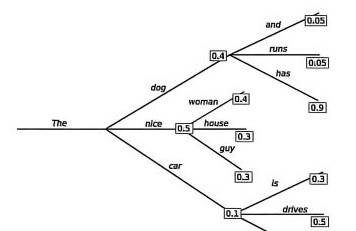
\includegraphics{images/image-0019.jpeg}
\caption{贪心搜索树状示例}
\end{figure}

问题：每步取最高≠乘积最高！

\Needspace{5\baselineskip}
\hypertarget{ux6ce2ux675fux641cux7d22}{%
\subsubsection{波束搜索}\label{ux6ce2ux675fux641cux7d22}}

波束搜索通过在每个时间步保留最可能的 \texttt{num\_beams} 个词，并从中最终选择出概率最高的序列，来降低丢失潜在高概率序列的风险。

波束搜索示例：图片展示了树状搜索过程。与贪心搜索不同，它在每一步会保留多个路径，例如 ``The nice'' 和 ``The dog''，然后继续扩展。

\begin{figure}[htbp]
\centering
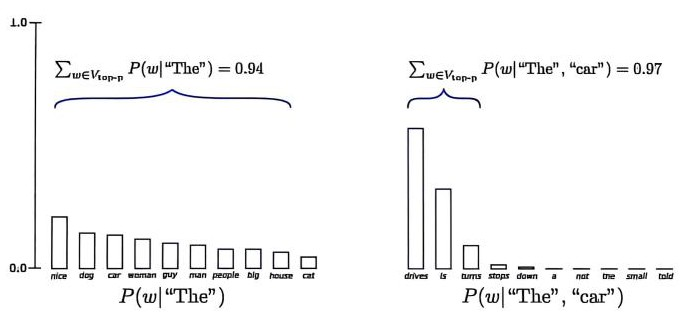
\includegraphics{images/image-0020.jpeg}
\caption{波束搜索树状示例}
\end{figure}

\textbf{Top-k 采样}：从概率最高的 \(k\) 个词中随机选择下一个词，平衡稳定性和多样性。

\[
S_k = \{x_i \mid P(x_i \mid x_1, x_2, \ldots, x_T) \mathcjk{ \mathcjk{是前} } k \mathcjk{ \mathcjk{高的}}\}
\]

\[
x_{T+1} \sim P(x_{T+1} \mid x_1, x_2, \ldots, x_T) \mathcjk{，\mathcjk{在} } S_k \mathcjk{ \mathcjk{中随机选择}}
\]

\textbf{Top-p 采样（Nucleus Sampling）}：从概率累积达到 \(p\) 的最小词集中随机选择下一个词，动态调整采样范围。

\[
S_p = \{x_i \mid \sum_{j=1}^{i} P(x_j \mid x_1, x_2, \ldots, x_T) \le p\}
\]

\[
x_{T+1} \sim P(x_{T+1} \mid x_1, x_2, \ldots, x_T) \mathcjk{，\mathcjk{在} } S_p \mathcjk{ \mathcjk{中随机选择}}
\]

\Needspace{5\baselineskip}
下面是Top-p采样的示意图：

\begin{figure}[htbp]
\centering
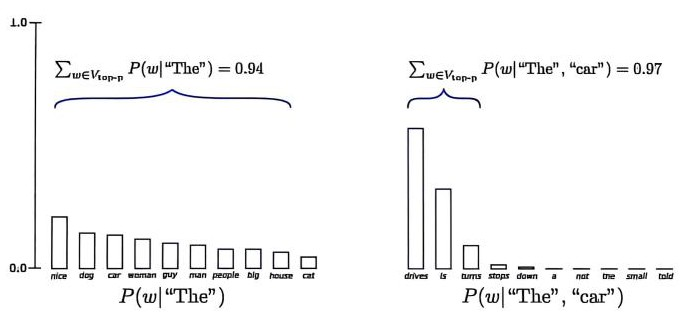
\includegraphics{images/image-0021.jpeg}
\caption{Top-p 采样分布示意图}
\end{figure}

也可以将Top-k与Top-p结合：先选K个，再从中选概率p。

\FloatBarrier
\Needspace{5\baselineskip}
\hypertarget{ux53c2ux8003ux6587ux732e-75}{%
\subsection{参考文献}\label{ux53c2ux8003ux6587ux732e-75}}

\vspace{0.25em}
\begin{itemize}
\tightlist
\item
  温睦宁、林江浩、张伟楠、俞勇（2025）。\href{https://haa.boyuai.com/}{《动手学大模型智能体》}。人民邮电出版社。ISBN 978-7-115-68638-1。
\item
  Holtzman, A., Buys, J., Du, L., Forbes, M., \& Choi, Y. (2020). \href{https://arxiv.org/abs/1904.09751}{The Curious Case of Neural Text Degeneration}. ICLR 2020.
\end{itemize}

\clearpage
